\documentclass{article}

%% PAQUETES

% Paquetes generales
\usepackage[margin=2cm, paperwidth=210mm, paperheight=297mm]{geometry}
\usepackage[spanish]{babel}
\usepackage[utf8]{inputenc}
\usepackage{gensymb}

% Paquetes para estilos
\usepackage{textcomp}
\usepackage{setspace}
\usepackage{colortbl}
\usepackage{color}
\usepackage{color}
\usepackage{upquote}
\usepackage{xcolor}
\usepackage{listings}
\usepackage{caption}
\usepackage[T1]{fontenc}
\usepackage[scaled]{beramono}

% Paquetes extras
\usepackage{amssymb}
\usepackage{float}
\usepackage{graphicx}
\usepackage{url}
\usepackage[toc,page]{appendix}
\usepackage{mips}


%% Fin PAQUETES


% Definición de preferencias para la impresión de código fuente.
%% Colores
\definecolor{gray99}{gray}{.99}
\definecolor{gray95}{gray}{.95}
\definecolor{gray75}{gray}{.75}
\definecolor{gray50}{gray}{.50}
\definecolor{keywords_blue}{rgb}{0.13,0.13,1}
\definecolor{comments_green}{rgb}{0,0.5,0}
\definecolor{strings_red}{rgb}{0.9,0,0}

%% Caja de código
\DeclareCaptionFont{white}{\color{white}}
\DeclareCaptionFont{style_labelfont}{\color{black}\textbf}
\DeclareCaptionFont{style_textfont}{\it\color{black}}
\DeclareCaptionFormat{listing}{\colorbox{gray95}{\parbox{16.78cm}{#1#2#3}}}
\captionsetup[lstlisting]{format=listing,labelfont=style_labelfont,textfont=style_textfont}

\lstset{
	aboveskip = {1.5\baselineskip},
	backgroundcolor = \color{gray99},
	basicstyle = \ttfamily\footnotesize,
	breakatwhitespace = true,   
	breaklines = true,
	captionpos = t,
	columns = fixed,
	commentstyle = \color{comments_green},
	escapeinside = {\%*}{*)}, 
	extendedchars = true,
	frame = lines,
	keywordstyle = \color{keywords_blue}\bfseries,
	language = C,                       
	numbers = left,
	numbersep = 5pt,
	numberstyle = \tiny\ttfamily\color{gray50},
	prebreak = \raisebox{0ex}[0ex][0ex]{\ensuremath{\hookleftarrow}},
	rulecolor = \color{gray75},
	showspaces = false,
	showstringspaces = false, 
	showtabs = false,
	stepnumber = 1,
	stringstyle = \color{strings_red},                                    
	tabsize = 2,
	title = \null, % Default value: title=\lstname
	upquote = true,                  
}

%% FIGURAS
\captionsetup[figure]{labelfont=bf,textfont=it}
%% TABLAS
\captionsetup[table]{labelfont=bf,textfont=it}

% COMANDOS

%% Titulo de las cajas de código
\renewcommand{\lstlistingname}{Código}
%% Titulo de las figuras
\renewcommand{\figurename}{Figura}
%% Titulo de las tablas
\renewcommand{\tablename}{Tabla}
%% Referencia a los códigos
\newcommand{\refcode}[1]{\textit{Código \ref{#1}}}
%% Referencia a las imagenes
\newcommand{\refimage}[1]{\textit{Imagen \ref{#1}}}

%% APENDICES
\addto\captionsspanish{
	\renewcommand\seename{Apéndices}
	\renewcommand\appendixname{Apéndices}
	\renewcommand\appendixpagename{Apéndices}
}


\begin{document}
\pagenumbering{roman}
\setcounter{page}{5}

% TÍTULO, AUTORES Y FECHA
\begin{titlepage}
	\vspace*{\fill}
	\begin{center}
		\Huge \textit{``Conjunto de instrucciones MIPS''} \\
		
		\bigskip\bigskip\bigskip\bigskip\bigskip

		\Large Federico Colangelo, Padrón Nro. 89.869 \\
		\large \textit{federico.colangelo@semperti.com} \\ \medskip
		\Large Facundo Rossi, Padrón Nro. 86.707 \\
		\large \textit{frossi85@gmail.com} \\ \medskip
		\Large Federico Martín Rossi, Padrón Nro. 92.086 \\
		\large \textit{federicomrossi@gmail.com} \\

		\bigskip\bigskip\bigskip\bigskip\bigskip\bigskip\bigskip

		\large 1er. Cuatrimestre 2013 \\ \smallskip
		\large 66.20 Organización de Computadoras \\ \smallskip
		\large Facultad de Ingeniería, Universidad de Buenos Aires \\ \smallskip

		\date{}
	\end{center}
	\vspace*{\fill}
\end{titlepage}

\newpage
\newpage \textit{}
\newpage



% ÍNDICE
\tableofcontents
\newpage \textit{}
\newpage
\pagenumbering{arabic}




% Introducción
\section{Introducción}
	
	En este trabajo presentamos la comparación entre dos algoritmos de ordenamiento:  el \textit{Bubblesort} y el \textit{Shellsort}.
	\par
	Para realizar la comparación entre ambos se realizó la implementación en lenguaje C de cada uno. A su vez, para comparar la performance entre código de alto nivel y código nativo, se hizo la implementación de shellsort en assembler MIPS, con el fin de poder comparar los tiempos de ejecución de ambos programas.
	\par
	Todo el trabajo se realizo en una plataforma \textit{NetBSD/MIPS-32} mediante el \textit{GXEmul} \cite{GXEMUL}
	\par
	Todos los archivos y códigos fuente aquí mencionados, así como también el presente informe, pueden ser
descargados de la sección Downloads del repositorio del grupo\footnote{URI del Repositorio: \url{https://code.google.com/p/tp-orga-computadoras/ }}.
\bigskip




% Compilación
\section{Compilación}
	
	La herramienta para compilar tanto el código asembly como C será el \textit{GCC} \cite{GCC}. Para tratar de equiparar al máximo el \textit{S} generado por ambas implementaciones, se utilizará el flag de gcc ``-O0'' para que no realice optimizaciones sobre el código en lenguaje C.
	\par
	Para automatizar las tareas de compilación se hace uso de la herramienta \textit{GNU Make} . Los Makefiles utilizados para la compilación se incluyen junto al resto de los archivos fuentes del presente trabajo \footnote{Los archivos se encuentran separados según la implemetación a la que pertenecen, por lo que habrán dos Makefiles distintos, uno para la implementación en lenguaje C y otro para la implementación en assembly}.
\bigskip




% Utilización
\section{Utilización}
	
	En los siguientes apartados se especifica la forma en la que deben ser ejecutados los programas implementados tanto en C como en assembly.
\medskip


\subsection{Implementación en C}

	El resultado de compilación con ``make'' será un programa ejecutable, de nombre \textit{tp0}, que podrá ser invocado con los siguientes parámetros:
\medskip

\begin{itemize}

\itemsep=2pt \topsep=0pt \partopsep=0pt \parskip=0pt \parsep=0pt
	\item \textit{-h}:  Imprime ayuda para la utilización del programa;
	\item \textit{-V}:  Imprimer la versión actual del programa;
	\item \textit{-b [ARGS]}:  El programa recibe nombres de archivos de texto o strings ingresados por \textit{stdin}, ordenandolos utilizando el algoritmo bubblersort. Para utilizar \textit{stdin} deberá omitirse [ARGS] y luego introducir las palabras;
	\item \textit{-s [ARGS]}:  El programa recibe nombres de archivos de texto o strings ingresados por \textit{stdin}, ordenandolos utilizando el algoritmo shellsort. Para utilizar \textit{stdin} deberá omitirse [ARGS] y luego introducir las palabras.

\end{itemize}	
\medskip



\subsection{Implementación en Assembly}

	El resultado de compilación con ``make'' será un programa ejecutable, de nombre \textit{tp0}, el cual aceptará un archivo de texto como argumento y lo ordenará con el algoritmo Shellsort.
\medskip




% Implementación
\section{Implementaciones}
	
	En lo que sigue de la sección, se presentarán los códigos fuente de las implementaciones de los algoritmos. Aquellos lectores interesados en la implementación completa de los dos programas, pueden dirigirse a los apéndices ubicados al final del presente informe. Recordamos que se han separado las implementaciones en dos de manera de poder mantener un orden entre ambos.



\subsection{Implementación en C}

	La implementación del programa fue divida en los siguientes módulos:
	\medskip

\begin{itemize}

\itemsep=2pt \topsep=0pt \partopsep=0pt \parskip=0pt \parsep=0pt
	\item \textbf{tp0}: Programa principal responsable de interpretar los comandos pasados por la terminal de modo que realice las tareas solicitadas por el usuario. Su principal función es encadenar el funcionamiento de los otros módulos y mostrar por pantalla el resultado obtenido;
	\item \textbf{fileloader}: Módulo encargado de levantar un archivo de texto desde el filesystem y convertirlo en un array donde cada posición es una palabra. Permite además dimensionar el tamaño en memoria necesario para cargar todo el archivo como un arreglo de palabras;
	\item \textbf{bubblesort}: Módulo encargado de levantar un archivo de texto desde el filesystem y convertirlo en un array donde cada posición es una palabra. Permite además dimensionar el tamaño en memoria necesario para cargar todo el archivo como un arreglo de palabras;
	\item \textbf{shellsort}: Módulo encargado de implementar el algoritmo de shellsort. Recibe como paramentros un arreglo de palabras desordenado y el tamaño del mismo. Como resultado devuelve dicho arreglo ordenado.

\end{itemize}	
\medskip


% Algoritmo Bubblesort 
\subsubsection{Algoritmo \textit{Bubblesort}}

	En el \refcode{codeBSh} se muestra el header de la librería, donde se declara la función Bubblesort, mientras que en el \refcode{codeBSc} se muestra la definición de la librería.

% Código
\lstset{ language = C } % Cambiamos el lenguaje para que parsee en C
\lstinputlisting[label=codeBSh,caption=``bubblesort.h'']{../Codigo/c/bubblesort.h} 
\bigskip


% Código
\lstset{ language = C } % Cambiamos el lenguaje para que parsee en C
\lstinputlisting[label=codeBSc,caption=``bubblesort.c'']{../Codigo/c/bubblesort.c} 
\bigskip\bigskip




% Algoritmo Shellsort
\subsubsection{Algoritmo \textit{Shellsort}}

	En el \refcode{codeSSh} se muestra el header de la librería, donde se declara la función Shellsort, mientras que en el \refcode{codeSSc} se muestra la definición de la librería.

% Código
\lstset{ language = C } % Cambiamos el lenguaje para que parsee en C
\lstinputlisting[label=codeSSh,caption=``shellsort.h'']{../Codigo/c/shellsort.h} 
\bigskip


% Código
\lstset{ language = C } % Cambiamos el lenguaje para que parsee en C
\lstinputlisting[label=codeSSc,caption=``shellsort.c'']{../Codigo/c/shellsort.c} 
\bigskip\bigskip




\newpage
\subsection{Implementación en Assembly}

	La implementación del programa fue divida en los siguientes módulos:
	\medskip

\begin{itemize}

\itemsep=2pt \topsep=0pt \partopsep=0pt \parskip=0pt \parsep=0pt
	\item \textbf{tp0}: Solamente recibe un texto como argumento por linea de comandos y lo imprime ordenandolo mediante shellsort. Esta implementado en C;
	\item \textbf{fileloader}: Se utiliza el mismo de la otra implementación;
	\item \textbf{swap}: Función implementada en assembler para intercambiar el valor de dos registros recibidos como parametros;
	\item \textbf{compare}: Función similar a strcmp de C. Recibe dos argumentos de tipo texto y decide cual es el que precede alfabeticamente.
	\item \textbf{shellsort}: Implementación en assembler del algoritmo de ordenamiento.

\end{itemize}	
\medskip




% Algoritmo Shellsort
\subsubsection{Algoritmo \textit{Shellsort}}

	En el \refcode{codeSSaMED} se muestra la implementación en assembly del algoritmo Shellsort.

% Código
\lstset{ language = [mips]Assembler} % Cambiamos el lenguaje para que parsee en MIPS
\lstinputlisting[label=codeSSaMED,caption=``shellsort.S'']{../Codigo/assembly/shellsort.S} 
\bigskip\bigskip\medskip




% Debugging
\section{Debugging}
	
	Para analizar el correcto funcionamiento de los programas se crearon programas adhoc que fueran corroborando el correcto funcionamiento de cada uno de los modulos de manera individual. La idea era simular el concepto de test unitario de lenguajes de alto nivel.
	\par
	Una vez que todos los módulos funcionaban de la manera esperada, se utilizó el programa principal como test de integración.
Finalmente se utilizó la herramienta \textit{Valgrind} para realizar un análisis minucioso del uso de memoria, corrigiendo así las pérdidas de memoria que se presentaban en cada módulo.
\bigskip




% Pruebas
\section{Pruebas}

	Para realizar las pruebas de cada algoritmo se procesaron cuatro textos provistos por la cátedra. Estos son ``\textit{Alicia en el País de las Maravillas}'' (173kB), ``\textit{Beowulf}'' (220kB), una ``\textit{Enciclopedia}'' (643kB) y ``\textit{Don Quijote}'' (2147kB).
	\par
	A cada ejecución se le midió el tiempo de procesamiento mediante el comando \textit{GNU ``time''} \cite{TIME}. A continuación un ejemplo de su utilización:
\bigskip

{\ttfamily\footnotesize
\indent \$ time ./tp0 -b alice.txt\\}


\noindent Esto imprimirá por pantalla el tiempo de ejecución que fue tabulado para cada caso. En el \textit{Cuadro 1} se muestran los valores de tiempo obtenidos.
\bigskip\bigskip


% Tabla 1
\begin{table}[!hbt]
	\begin{center}
	\begin{tabular}{|>{\centering\arraybackslash}m{3cm}|>{\centering \arraybackslash}m{3cm}|>{\centering \arraybackslash}m{3cm}|>{\centering \arraybackslash}m{3cm}|}
		\hline
		\rowcolor[gray]{0.9}\textbf{Archivo de texto} & \textbf{bubblesort.c [s] } & \textbf{shellsort.c [s] }  & \textbf{shellsort.S [s] }\\
		\hline
		\centering alice.txt & 571,715 & 2,207 & 1,035  \\
		\hline
		\centering beowulf.txt & 958,527 & 3,418 & 1,500  \\
		\hline
		\centering cyclopedia.txt & >3600 & 12,184 & 6,914   \\
		\hline
		\centering elquijote.txt & >3600 & 48,957 & 33,098  \\
		\hline
	\end{tabular}
	\caption{Tiempos en segundos obtenidos en la ejecución de los distintos algoritmos.}
	\end{center}
\end{table}
\bigskip\bigskip


	En los graficos que siguen se muestran distintas comparaciones hechas con estos datos obtenidos, los cuales nos llevarán a la conclusión final.
\bigskip\bigskip

% Figura 1
\begin{figure}[h]
	\centering
	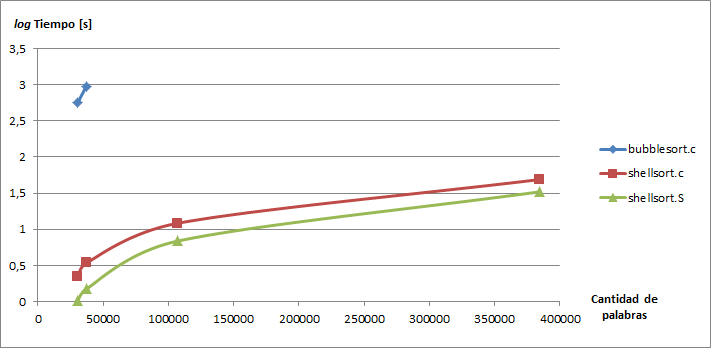
\includegraphics[width=0.85\textwidth]{images/imagen01.png}
	\medskip
	\caption{Gráfico de tiempo insumido (en segundos)  contra el\\ tamaño de la muestra (cantidad de palabras)}
\end{figure}

\newpage
% Figura 1
\begin{figure}[h]
	\centering
	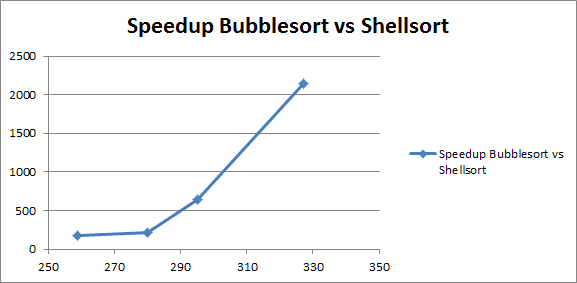
\includegraphics[width=0.85\textwidth]{images/imagen02.png}
	\medskip
	\caption{Gráfico del speedup del Bubblesort contra Shellsort\\ para los diversos tamaños de archivo.}
\end{figure}
\bigskip\bigskip


% Conclusiones
\section{Conclusiones}

	Al realizar la comparación entre los algoritmos bubblesort y shellsort en C, vemos que la diferencia entre ambos es notable. Estamos hablando de varios ordenes de maginitud.
	\par
	Esto se debe a que por su codigo bubblesort tiene un coste de O($n^2$) mientras que si bien no podemos determinarlo fácilmente para shellsort, ya que depende mucho del gap elegido, estamos hablando de algo cercano a O($n log(n)$). Esto hace que para textos grandes no sea una opción viable la utilización de bubblesort, mientras que shellsort prueba ser muy eficiente y el esfuerzo de codificación no es demsiado grande.
	\par
	En cuanto a la comparación de assembler y C, notamos una ligera ventaja del primero. Creemos que esto se debe a que muchas de las cosas que el algoritmo en C utiliza como variables en memoria principal, assembler utiliza registros los cuales presentan un tiempo de lecto/escritura notablemente menor.
\bigskip\bigskip




% Citas bibliográficas.
\begin{thebibliography}{99}

	\bibitem{GXEMUL} The NetBSD project, \url{http://www.netbsd.org/}

	\bibitem{GCC} GCC, the GNU Compiler Collection, \url{http://gcc.gnu.org/}

	\bibitem{BS} Bubblesort, \url{http://en.wikipedia.org/wiki/Bubble_sort}

	\bibitem{SS} Shellsort, \url{http://en.wikipedia.org/wiki/Shell_sort}

	\bibitem{TIME} time man page, \url{http://unixhelp.ed.ac.uk/CGI/man-cgi?time}

	\bibitem{ABI} MIPS ABI, \url{http://www.sco.com/developers/devspecs/mipsabi.pdf}

	\bibitem{HEN00} J. L. Hennessy and D. A. Patterson, ``Computer Architecture. A Quantitative
	Approach,'' 4th Edition, Morgan Kaufmann Publishers, 2000.

	\end{thebibliography}

\newpage


% Apendices
\begin{appendices}

\bigskip\bigskip

% Implementación completa en lenguaje C
\section{Implementación completa en lenguaje C}


\subsection{\textit{tp0.c}. Implementación del main del programa}
% Código
\lstset{ language = C } % Cambiamos el lenguaje para que parsee en C
\lstinputlisting[label=codeTP0cfull,caption=``tp0.c'']{../Codigo/c/tp0.c} 
\bigskip\bigskip

\subsection{\textit{bubblesort.h}. Declaración de la librería Bubblesort}
% Código
\lstset{ language = C } % Cambiamos el lenguaje para que parsee en C
\lstinputlisting[label=codeBShfull,caption=``bubblesort.h'']{../Codigo/c/bubblesort.h} 
\bigskip\bigskip

\subsection{\textit{bubblesort.c}. Definición de la librería Bubblesort}
% Código
\lstset{ language = C } % Cambiamos el lenguaje para que parsee en C
\lstinputlisting[label=codeBScfull,caption=``bubblesort.c'']{../Codigo/c/bubblesort.c} 
\bigskip\bigskip

\subsection{\textit{shellsort.h}. Declaración de la librería Shellsort}
% Código
\lstset{ language = C } % Cambiamos el lenguaje para que parsee en C
\lstinputlisting[label=codeSShfull,caption=``shellsort.h'']{../Codigo/c/shellsort.h} 
\bigskip\bigskip

\subsection{\textit{shellsort.c}. Definición de la librería Shellsort}
% Código
\lstset{ language = C } % Cambiamos el lenguaje para que parsee en C
\lstinputlisting[label=codeSScfull,caption=``shellsort.c'']{../Codigo/c/shellsort.c} 
\bigskip\bigskip

\subsection{\textit{fileloader.h}. Declaración de la librería File Loader}
% Código
\lstset{ language = C } % Cambiamos el lenguaje para que parsee en C
\lstinputlisting[label=codeFLhfull,caption=``fileloader.h'']{../Codigo/c/fileloader.h} 
\bigskip\bigskip

\subsection{\textit{fileloader.c}. Definición de la librería File Loader}
% Código
\lstset{ language = C } % Cambiamos el lenguaje para que parsee en C
\lstinputlisting[label=codeFLcfull,caption=``fileloader.c'']{../Codigo/c/fileloader.c} 
\bigskip\bigskip




% Implementación completa en assembly MIPS
\section{Implementación completa de Shellsort en assembly MIPS}


\subsection{\textit{tp0.c}. Implementación del main del programa}
% Código
\lstset{ language = C } % Cambiamos el lenguaje para que parsee en C
\lstinputlisting[label=codeTP0afull,caption=``tp0.c'']{../Codigo/assembly/tp0.c} 
\bigskip\bigskip

\subsection{\textit{shellsort.S}. Implementación del algoritmo Shellsort}
% Código
\lstset{ language = [mips]Assembler} % Cambiamos el lenguaje para que parsee en MIPS
\lstinputlisting[label=codeSSafull,caption=``shellsort.S'']{../Codigo/assembly/shellsort.S} 
\bigskip\bigskip

\subsection{\textit{compare.S}. Implementación del comparador de palabras}
% Código
\lstset{ language = [mips]Assembler} % Cambiamos el lenguaje para que parsee en MIPS
\lstinputlisting[label=codeCMPafull,caption=``compare.S'']{../Codigo/assembly/compare.S} 
\bigskip\bigskip

\subsection{\textit{swap.S}. Implementación del comparador de palabras}
% Código
\lstset{ language = [mips]Assembler} % Cambiamos el lenguaje para que parsee en MIPS
\lstinputlisting[label=codeSWAPafull,caption=``swap.S'']{../Codigo/assembly/swap.S} 
\bigskip\bigskip


\end{appendices}

\end{document}
